\chapter{\label{a3-extractors}Charge Extractor Investigations}

\minitoc

\notes[inline,caption={}]{
	\section{Plan}
	\subsection{Topics}
	\begin{itemize}
		\item RMS extracted charge with varying integration window size and shift with different NSBs and amplitudes (and combination of amplitudes)
		\item Charge resolution of different methods with different NSB (including full integration method)
		\item in the absence of the need for peak finding (laser illumination), and when peak finding is important (Cherenkov) - split into two, best integration technique (different NSBs, different integration window sizes), and best peak finding (different NSBs, need Cherenkov data)
		\item window size might actually change for Cherenkov - got to capture entire signal, and signal might not be centred at "calculated peak time".
	\end{itemize}
	\subsection{Questions}
	\begin{itemize}
		\item ?
	\end{itemize}
}

\section{Introduction}

In Chapter~\ref{ch6-reduction}, the different algorithms for extracting charge from a waveform is extensively discussed, as well as the important considerations one must be vigilant of. This Appendix is provided to inform about the performance of the chosen charge extraction approaches, \textit{Cross Correlation} and \textit{Neighbour Peak Finding}, in comparison to typical charge extraction approaches, in the context of \gls{chec-s}.

\section{Integration Window}

\begin{figure}
  \begin{subfigure}[b]{0.49\textwidth}
    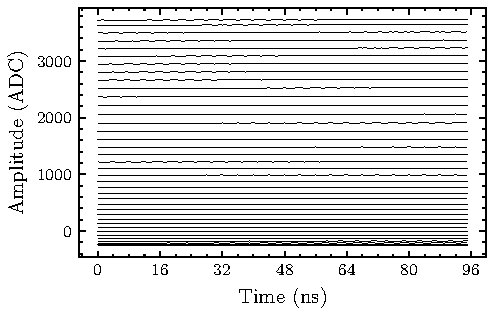
\includegraphics[width=\textwidth]{generation_t5}
    \caption{DC Transfer Function input, measured with TARGET~5.}
    \label{fig:generation_t5}
  \end{subfigure}
  \hfill
  \begin{subfigure}[b]{0.49\textwidth}
    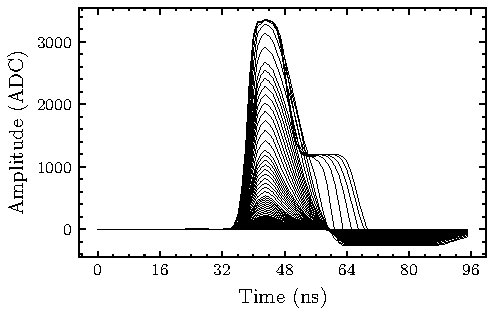
\includegraphics[width=\textwidth]{generation_tc}
    \caption{AC Transfer Function input, measured with TARGET~C.}
    \label{fig:generation_tc}
  \end{subfigure}
  \caption[Transfer Function generation waveforms.]{Multiple average waveforms, increasing in amplitude. Each average contains 1000 waveforms from the same single channel. These waveforms cover the full dynamic range of the TARGET ASIC, and are used as inputs to generate the DC and AC Transfer Functions, respectively. The saturation behaviour of the TARGET C ASIC can be seen in the high amplitude waveforms in (b).}
\end{figure}

As an alternative to the \textit{Cross Correlation} integration approach, one may instead use a simple integration window, defined by its ``window width'' and the ``shift'' from the peak time. The first step in this investigation is to find the optimal values for the width and shift of the window when extracting charge from a \gls{chec-s} waveform. This exercise is performed using a Monte Carlo simulation of the lab set-up, where the camera is uniformly illuminated. As the pulse time is consistent in this simulation, it allows the investigation to be solely on the integration approach, avoiding the contributions of peak finding.









